\documentclass[../main.tex]{subfiles}
\begin{document}
\chapter{Moon Cloud: un framework per il monitoraggio e la security assurance}
\section{Introduzione}
In questo capitolo verrà approfondito Moon Cloud\footnote{MOnitoring and assurance ON Cloud, \textit{https://www.moon-cloud.eu/}}, un framework per il monitoraggio e l'assurance di sistemi tradizionali, cloud e Internet of Things, sviluppato dal laboratorio SESAR Lab\footnote{SEcure Service-oriented Architectures Research Lab - \textit{http://sesar.di.unimi.it}} dell'Università degli Studi di Milano.

L'obiettivo del progetto Moon Cloud è quello di implementare una metodologia automatica per la valutazione della sicurezza, delle performance e di altre proprietà non funzionali, offrendo un processo di assurance basato su attività di auditing e raccolta di evidenze.

Le caratteristiche di Moon Cloud sono le seguenti\cite{MoonCloudWebsite}:
\begin{itemize}
    \item \textbf{Framework automatico e personalizzabile orientato a microservizi} basato su modelli per la raccolta di evidenze
    \item \textbf{Copertura di tutto lo stack cloud}, ai livelli \textit{IaaS}, \textit{PaaS}, \textit{SaaS}
    \item \textbf{Possibilità di integrazione con tecnologie pre-esistenti e di terze parti}
\end{itemize}

L'orchestrazione avviene tramite una  \textit{dashboard} grafica erogata in modalità \textit{Software as-a-Service}, la quale si interfaccia con diversi componenti che ne implementano la logica di funzionamento, l'esecuzione dei test, il collezionamento dei risultati e il reporting dello stato di compliance del sistema analizzato.

Moon Cloud nasce sulla scia del progetto europeo FP7 CUMULUS - il cui obiettivo è quello di fornire un framework per la certificazione di servizi cloud mediante l'assessment di proprietà non funzionali\cite{CumulusBigDoc} - da cui riprende alcune caratteristiche architetturali. 

L'obiettivo di questo capitolo è quello di dare al lettore il \texit{know-how} necessario a comprendere le motivazioni di alcune decisioni prese nella realizzazione della tesi, in particolar modo per gestire alcune limitazioni del framework Moon Cloud. 
Di seguito sarà proposta una breve panoramica sulla terminologia utilizzata, sulle componenti principali,  e sui principi di funzionamento dei processi di \textit{assessment} e \textit{compliance} all'interno della piattaforma.


\section{Terminologia}
\begin{itemize}
    \item \textbf{Metriche}: insieme di proprietà non funzionali di cui si vogliono ottenere \textbf{misurazioni}.
    \item \textbf{Controllo}: rappresenta la modalità di raccolta ed elaborazione delle \textit{misurazioni} di una \textit{metrica}.
        Esso è descritto tramite un documento \textit{JSON}\footnote{JSON, JavaScript Object Notation, \textit{http://www.json.org/}}, i cui attributi sono
        \begin{itemize}
            \item \textbf{name}, nome del controllo
            \item \textbf{description}, descrizione del controllo
            \item \textbf{category}, categoria di appartenenza
            \item \textbf{driver-name}, nome del driver che ne implementa il flusso di esecuzione
            \item \textbf{inputs}, dati ricevuti in input
            \item \textbf{outputs}, dati attesi in output (\textit{misurazioni})
        \end{itemize}
    \item \textbf{Driver}: la porzione di codice che implementa il controllo 
    \item \textbf{Test}: istanza di un controllo, che ne rappresenta l'esecuzione con gli input effettivi 
    \item \textbf{Regola di valutazione astratta}, o \textit{AER (abstract evaluation rule)}, regola logica che implementa un processo di compliance. È data dall'aggregazione di controlli mediante operatori \textit{booleani}. I suoi termini possono essere \textit{controlli} e altre \textit{AER}.
    \item \textbf{Regola di valutazione concreta}, o \textit{ER (evaluation rule)}: istanza di una \textit{AER}. I suoi termini possono essere \textit{test} (mappati sui rispettivi \textit{controlli} o altre \textit{ER}.
\end{itemize}
\vfill
\newpage

\section{Architettura e componenti}
\begin{figure}[H]
\centering
\makebox[\textwidth]{
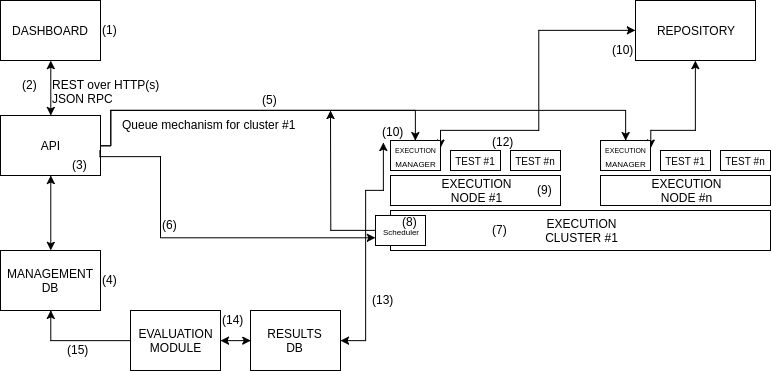
\includegraphics[width=\textwidth]{immagini/MCArchi.png}
}
\caption{Architettura e componenti di Moon Cloud}\label{fig:MCArchi}
\end{figure}
In figura \ref{fig:MCArchi} sono illustrate l'architettura del framework Moon Cloud e l'interazione tra i vari microservizi che lo compongono.
Questa può essere divisa in due aree. La prima, accessibile dagli utenti del sistema fornisce le funzionalità di gestione e comprende:
\begin{itemize}
    \item \textbf{Dashboard} (1), sviluppata in Javascript, HTML5 e CSS mediante il framework Angular.JS. Rappresenta il punto di ingresso per l'utente, e fornisce un'interfaccia grafica per la fruizione delle funzionalità del prodotto. La \textit{Dashboard} è supportata da API HTTP servite in modo sicuro tramite il protocollo TLS (2).
    \item \textbf{API} (3), costituiscono l'intefaccia con le principali funzionalità del sistema. Interagiscono con un database di management (4) seguendo il paradigma RESTful, e orchestrano l'esecuzione dei test.
        Il test può essere lanciato:
        \begin{itemize}
            \item inviando un messaggio agli \textit{execution manager} (9) mediante un meccanismo di comunicazione basato su code(5).
            \item inserendo un \textit{task} periodico(6) nello \textit{scheduler} (7)
        \end{itemize}
\end{itemize}
La seconda invece, rappresenta il vero e proprio backend del framework, gestendo i meccanismi di esecuzione dei test, raccolta dei risultati e valutazione degli stessi.
È composta da:
\begin{itemize}
    \item \textbf{Execution Cluster} (8), ovvero l'insieme dei nodi - \textit{execution node}, (9)  - che eseguono materialmente il test. I cluster sono equipaggiati da uno \textit{scheduler} (7), che gestisce l'esecuzione temporizzata dei test periodici, per effettuare il monitoraggio in modo continuo, inviando i test in esso memorizzati a cadenze temporali scandite da un pattern \textit{CRON}\footnote{http://man7.org/linux/man-pages/man5/crontab.5.html}.
    \item \textbf{Execution Manager} (10), ovvero il servizio che gestisce il lavoro di ciascun nodo del cluster.        
        Gli \textit{execution manager} di uno stesso cluster sono connessi alla stessa coda: all'arrivo di un messaggio essi ne effettuano il \textit{prefetch}, ne validano il contenuto, effettuano il download il driver relativo al controllo referenziato dal test dal repository (11), eseguono lo stesso con gli input contenuti nel messaggio, e collezionano gli output del test in un database non relazionale \textit{time series}(12).
    \item \textbf{Evaluation Module} (13), rimane in ascolto sul database \textit{time-series} (12) in attesa di eventi. Quando lo stato di uno specifico test cambia, avvia la procedura di valutazione di tutte le \textit{ER} che fanno riferimento a tale test, e ne memorizza il risultato nel database di management (4).
    \item \textbf{Repository} (10), contiene i driver per i controlli di sicurezza. È realizzato tramite un ambiente Git\footnote{Git, \textit{https://git-scm.com/}}, di cui condivide le funzionalità, e da un \textit{registry} di \textit{container}, che rappresentano il singolo driver. Il processo di sviluppo di un driver è ultimato da un motore di \textit{continuous integration} che contestualmente al caricamento del codice dello stesso sul \textit{repository} effettua la build del \textit{container} associato e test automatici di validazione e sanitizzazione dello stesso, per poi pubblicare il \textit{container} sul \textit{registry}..
\end{itemize}
\section{Moon Cloud come strumento di verifica delle \textit{recommendation}}

La verifica delle \textit{recommendation} è il processo di verifica della conformità di un sistema target ad una data raccomandazione.
Si tratta di un processo complesso, poiché può richiedere l'aggregazione dei risultati delle valutazioni di diversi servizi; nel caso di Moon Cloud, il processo di valutazione è effettuato tramite la raccolta di evidenze, mediante tecniche di testing e monitoraggio su uno specifico servizio. 
Le evidenze vengono poi utilizzate per verificare se la raccomandazione sia effettivamente rispettata o no.

\begin{definition}[Recommendation verification]\label{def:prop}
    Sia $\Rec{}$ la \textit{recommendation} da verificare, la \textit{reccomendation verification} è una funzione $\widehat{\Rec{}}$ definita sulla tupla $\langle$$\EP{}$, $\ER{}$$\rangle$ che restituisce un valore booleano \{true, false\} dove:
\begin{itemize}
    \item $\EP{}$ è l'insieme di \textit{processi di valutazione} \{$\Eval{}$\} da eseguire. L'\textit{output} del processo di valutazione è un valore \textit{booleano} che espreime se la valutazione abbia avuto successo o no, aggregato alle \textit{evidence} collezionate a supporto del risultato.
        \item $\ER{}$ is an \textit{evaluation rule} expressed as a propositional logic formula in terms of the evaluation processes $\Eval{}$. It combines the results of the different evaluations $\Eval{}$$\in$$\EP{}$ and returns true if the property is positively evaluated, false otherwise.
\end{itemize}
\end{definition}
We note that, although we can implement more complex first order logic formulas for $\ER{}$, propositional logic provides enough expression power to cover all the recommendations in Section~\ref{sec:bench}.

% bisogna rifare per una recommandation di quelle fatte sopra
An evaluation process $\Eval{}$$\in$$EP{}$ refers to the evaluation of a specific service.
%Each evaluation process $Eval\in E$ drives the moon cloud architecture instrumenting a specific evaluation setting up the relative evidence collection. They are defined as follows. 
\begin{definition}[$\Eval{}$]\label{def:eval}
An evaluation process $\Eval{}$ is a tuple of the form $\langle$$t$, $C$$\rangle$, where:
\begin{itemize}
	\item $t$ is the \emph{ToE (Target of Evaluation)}. It is defined as the services constituting the perimeter of the evaluation. 
	%Controlli come funzione
	\item $C$ is the \emph{Control}, that is, the process executing the evaluation on $t$ and returning the result of the evaluation together with the set of collected evidence.
\end{itemize}
\end{definition}

We note that the ToE can be either a public service or a specific mechanism providing a security feature to be evaluated.

A Control $C$ defines details on how to collect evidence on a specific target $t$ to evaluate a recommendation. It is defined as follows.
\begin{definition}[$C$]\label{def:control}
$C$ is defined over a 3-tuple of the form $\langle$$\phi$, $\lambda$, $\pi$$\rangle$, where:
\begin{itemize}
	\item $\phi$ is the flow of evidence collection execution. It is composed of a sequence of atomic evaluation operations.
	\item $\lambda$ is set of \textit{Control's Parameters} necessary to connect the evaluation flow $\phi$ to the target service $t$ (e.g., the target URI)
	\item $\pi$ is a set of \textit{Environmental Settings} describing how to deploy the control (e.g., within the ToE perimeter or not) and possible dependencies on its execution. 
\end{itemize}
\end{definition}

The execution of a given Control returns true or false plus a set of evidence on its execution, which are collected at recommendation verification level.



Moon Cloud implements the recommendation verification process in Section~\ref{sec:basic} to assess cloud systems security. 
It is able to execute a number of evaluation processes $\Eval{}$ in parallel, each one referring to a set of recommendations $\Rec{}$ to be evaluated. 
It models controls $C$ in Section~\ref{sec:basic} using skeletons. The code/execution flow ($\phi$) is modeled as a chain containing all operations the control needs to exercise for evidence collection.\footnote{The flow $\phi$ can be serialized as a sequence of operations.} It is implemented as python script. We note that the first operation of the chain is the configuration of the target service using parameters $\lambda$. 
Parameters ($\lambda$) and Environment ($\pi$) are represented using a meta-data format. Each operation within the control flow $\phi$ is connected to the specific parameters needed for the evaluation, while environment $\pi$ represents the set of pre-requisites and dependencies to execute or deploy the specific control. Figure~\ref{fig:script} shows the code/execution flow $\phi$ as a python script for $C_{2}$ in Example~\ref{C:example}.
%esempio di come sono codificati parametri ed environment potrebbe essere utile

\subsection{Driver per i controlli di sicurezza}
\subsubsection{Struttura di un driver}
\subsubsection{Meccanismo di \textit{continuous integration}}
\subsubsection{Payload del driver}
\subsection{Regole di valutazione}
\subsubsection{Regole di valutazione astratte}
\subsubsection{Regole di valutazione concrete}
\end{document}
